\section{Introduction}
\label{sec:intro}

% To insert a figure: % Use figure* for multi-column figure
\begin{figure}[tp]
    \centering
    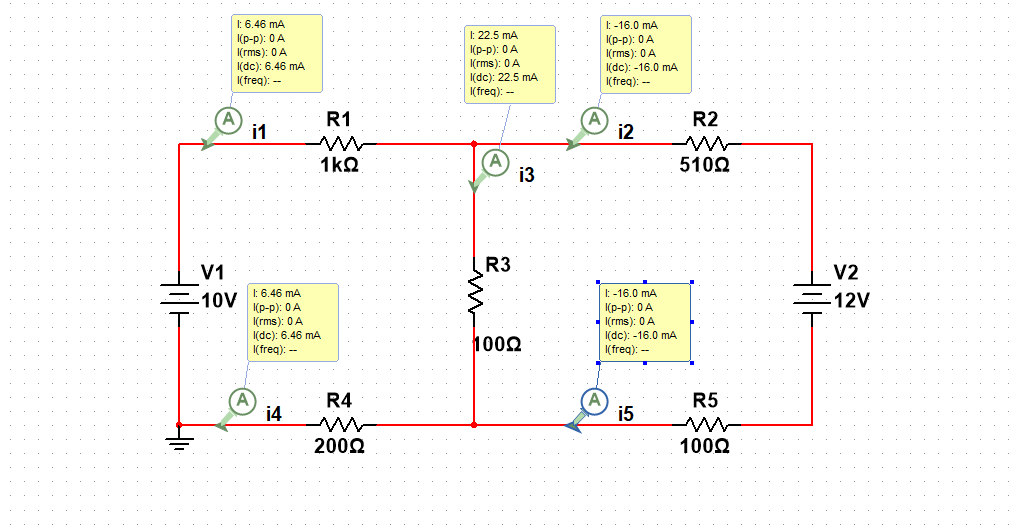
\includegraphics[width=\linewidth]{figs/demo.png}
    \caption{Caption.}
    \label{fig:template}
\end{figure}

% Or table: % Use figure* for multi-column figure
\begin{figure}[tp]
    \centering
    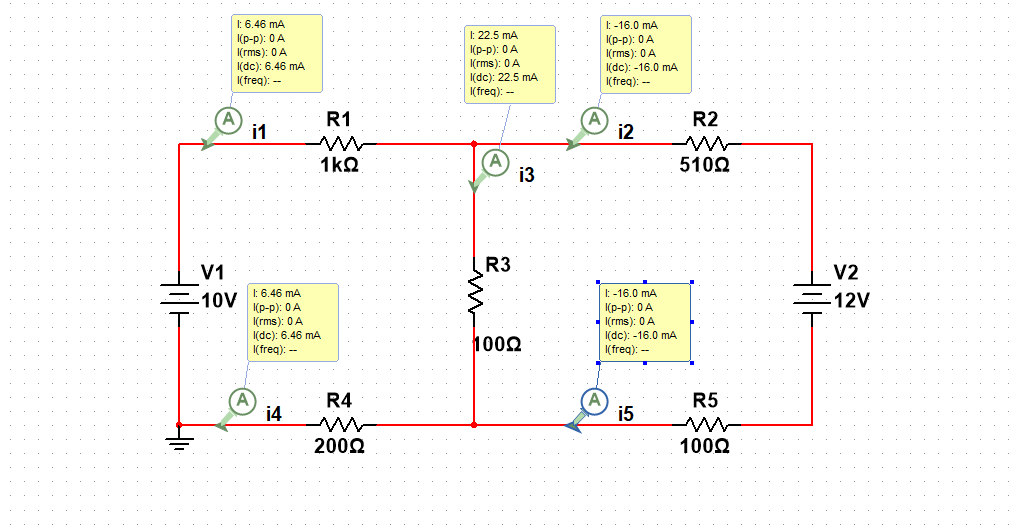
\includegraphics[width=\linewidth]{figs/demo.png}
    \caption{Caption.}
    \label{fig:template}
\end{figure}


hello,this is a demo. In this project, we use a method called "Funny" to enable the cow can fly in the sky and under the cow all of the cow say "wow! there is must a man are traying."

hello,this is a demo. In this project, we use a method called "Funny" to enable the cow can fly in the sky and under the cow all of the cow say "wow! there is must a man are traying."

hello,this is a demo. In this project, we use a method called "Funny" to enable the cow can fly in the sky and under the cow all of the cow say "wow! there is must a man are traying."

hello,this is a demo. In this project, we use a method called "Funny" to enable the cow can fly in the sky and under the cow all of the cow say "wow! there is must a man are traying."

hello,this is a demo. In this project, we use a method called "Funny" to enable the cow can fly in the sky and under the cow all of the cow say "wow! there is must a man are traying."

hello,this is a demo. In this project, we use a method called "Funny" to enable the cow can fly in the sky and under the cow all of the cow say "wow! there is must a man are traying."

hello,this is a demo. In this project, we use a method called "Funny" to enable the cow can fly in the sky and under the cow all of the cow say "wow! there is must a man are traying."

hello,this is a demo. In this project, we use a method called "Funny" to enable the cow can fly in the sky and under the cow all of the cow say "wow! there is must a man are traying."

% Use figure* for multi-column figure
\begin{figure}[tp]
    \centering
    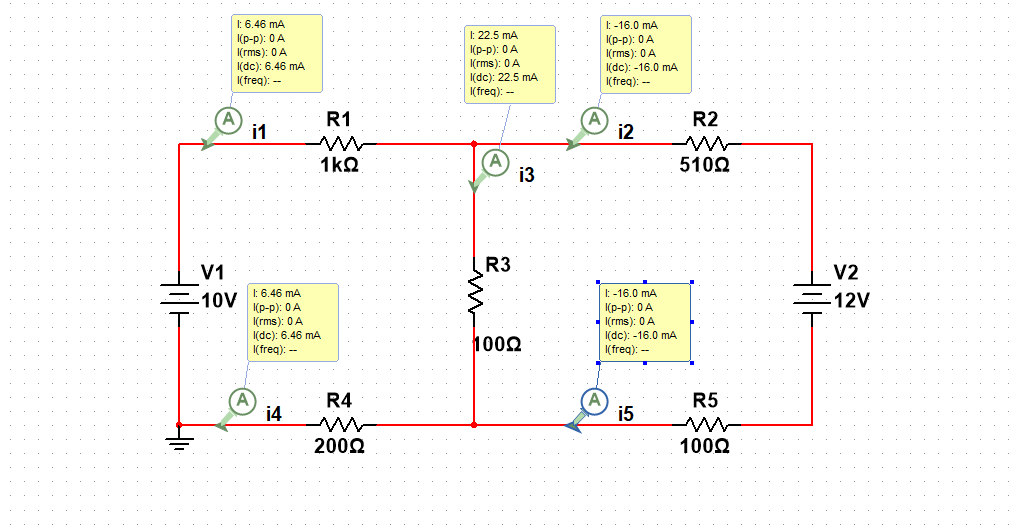
\includegraphics[width=\linewidth]{figs/demo.png}
    \caption{Caption.}
    \label{fig:template}
\end{figure}
